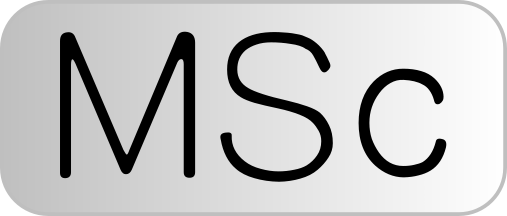
\includegraphics[height=1.25cm]{images/pictograms/msc}

\includegraphics[height=1.25cm]{images/pictograms/FEM}
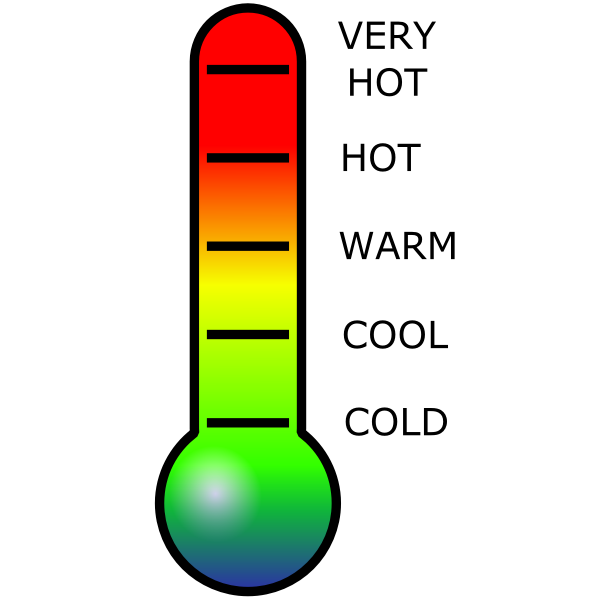
\includegraphics[height=1.25cm]{images/pictograms/temperature}

%%%%%%%%%%%%%%%%%%%%%%%%%%%%%%%%%%%%%%%%%%%%%%%%%%%%%%%%%%%%%%%%%%%%%%%%%%%%%%%%%%%%%%%%%%%%%%%%%%%


\lstinputlisting[language=bash,basicstyle=\small]{python_codes/fieldstone_33/keywords.ascii}

\begin{center}
Code at \url{https://github.com/cedrict/fieldstone/tree/master/python_codes/fieldstone_33}
\end{center}

\par\noindent\rule{\textwidth}{0.4pt}

{\sl This fieldstone was developed in collaboration with Rens Elbertsen}. \index{contributors}{R. Elbertsen}

\par\noindent\rule{\textwidth}{0.4pt}

%%%%%%%%%%%%%%%%%%%%%%%%%%%%%%%%%%%%%%%%%%%%%%%%%%%%%%%%%%%%%%%%%%%%%%%%%%%%%%%%%%%%%%%%%%%%%%%%%%%%


This is based on the community benchmark for viscoplastic thermal convection
in a 2D square box (Tosi et al (2015) \cite{tosn15}) as already carried out in \stone~28.

In this experiment the geometry is an annulus of inner radius 
$R_1=1.22$ and outer radius $R_2=2.22$. 
The rheology and buoyancy forces are identical to those of the box 
experiment. The initial temperature is now given by:
\[
T(r,\theta) = T_c(r)+A\; s(1-s) \cos(N_0 \theta)
\quad\quad s=\frac{R_2-r}{R_2-R_1} \in [0,1]
\]
where $s$ in the normalised depth, $A$ is the amplitude of the perturbation and $N_0$ the 
number of lobes. In this equation $T_c(r)$ stands for the steady state purely conductive 
temperature solution which is obtained by solving the Laplace's equation in 
polar coordinates (all terms in $\theta$ are dropped because of radial symmetry) 
supplemented with two boundary conditions:
\[
\Delta T_c = \frac{1}{r}\frac{\partial }{\partial r} \left( r \frac{\partial T}{\partial r} \right) =0 
\quad\quad
\quad\quad
T(r=R_1)=T_1=1
\quad\quad
\quad\quad
T(r=R_2)=T_2=0
\]
We obtain 
\[
T_c(r)=\frac{\log (r/R_2)}{\log(R_1/R_2)}
\]
Note that this profile differs from the straight line that is used in Tosi \etal (2015) \cite{tosn15} 
and in \stone~28.

\begin{center}
\includegraphics[width=5.5cm]{python_codes/fieldstone_33/images/T_N03}
\includegraphics[width=5.5cm]{python_codes/fieldstone_33/images/T_N05}
\includegraphics[width=5.5cm]{python_codes/fieldstone_33/images/T_N11}\\
{\captionfont Examples of initial temperature fields for $N_0=3,5,11$}
\end{center}

Boundary conditions can be either no-slip or free-slip on both inner and outer boundary. 
However, when free-slip is used on both a velocity null space exists and must be filtered out:
the solution contains an arbitrary rotation on top of the solution we are interested in.
This additional velocity field can be problematic since velocity enters the advection-diffusion 
equation for temperature (and/or compositions)
and it also essentially determines the time step value for a chosen mesh size (CFL condition).

Only the number of elements $nelr$ in the radial direction can be chosen by the user
since the number of elements in the tangential direction $nelt$ is automatically determined
such that elements at the surface of the annulus are approximately square.

%........................................................
\paragraph{About the nullspace}
For these reasons the nullspace must be removed from the obtained solution after every timestep.
There are two types of nullspace removal: removing net angular momentum, and removing net rotations.
The technique that we use here is simple:
\begin{enumerate}
\item pin the first node which is at position ($x=R_1,y=0$) by prescribing its vertical velocity to zero. This 
eliminates the nullspace completely. 
\item compute the angular momentum and correct the velocity field so that it is zero as explained in section \ref{ss_nullspace}.


%We calculate at each time step (at each non linear iteration) the average angular velocity ${\vec\omega}$ 
%of the cylindrical shell:
%\[
%<{\vec\omega}> = \frac{1}{V} \int_V \frac{{\vec r}\times {\vec\upnu}}{r^2} dV
%\]
%where $V$ is the shell volume and ${\bm r}$ the position vector. 
%In this case, we have $\vec{r}=(x,y,0)$ and $\upnu=(u,v,0)$ so that 
%${\vec r}\times {\vec\upnu}=(0,0,xv-uy)$.
The corrected velocity field $\vec{\upnu}'$ is then given by 
\[
\vec{\upnu}' = \vec{\upnu} - <\vec\omega>\times \vec{r}
\]
and it is easy to verify that 
\begin{eqnarray}
<{\vec\omega}'> 
&=& \frac{1}{V} \int_V \frac{{\vec r}\times {\vec\upnu}'}{r^2} dV \nn\\
&=& \frac{1}{V} \int_V \frac{{\vec r}\times (\vec{\upnu} - <\vec\omega>\times \vec{r})   }{r^2} dV\nn\\
&=& \frac{1}{V} \int_V \frac{{\vec r}\times \vec{\upnu}    }{r^2} dV
- \frac{1}{V} \int_V \frac{{\vec r}\times  <\vec\omega>\times \vec{r}   }{r^2} dV\nn\\
&=&  <{\vec\omega}> -  <{\vec\omega}> \frac{1}{V} \int_V dV = 0
\end{eqnarray}

\end{enumerate}



%........................................................
\paragraph{Measurements} We calculate and monitor the following quantities:
\begin{itemize}
\item the average temperature $<T>$
\begin{equation}
\langle T \rangle = \frac{\int_\Omega T  d\Omega }{\int_\Omega d \Omega }
=\frac{1}{V_\Omega}\int_\Omega T d\Omega
\end{equation}
\item the root mean square velocity $v_{rms}$ as given by equation (\ref{MMM-eqVrms}).
\item the root mean square of the radial and tangential velocity components as given 
by equations (\ref{eqVrVrms}) and (\ref{eqThetaVrms}).
\item the heat transfer through both boundaries $Q$:
\begin{equation}
Q_{inner, outer} = \int_{\Gamma_{i,o}} \boldsymbol{q} \cdot \boldsymbol{{n}} \; d\Gamma 
\end{equation}
\item the Nusselt number at both boundaries $\Nunb$ as given by equations 
(\ref{eqNuAnnIn}) and  (\ref{eqNuAnnOut}). 
\item the power spectrum of the temperature field:
\begin{equation}
PS_n(T) = \left |\int_\Omega T(r, \theta) e^{in\theta} d\Omega \right |^2.
\end{equation}
\item the average viscosity $\langle \eta \rangle$ (see Eq.~\ref{eq:avrgeta})
\end{itemize}

%........................................................
\paragraph{Cases and rheologies}
In the following Table, we list the benchmark cases according to the parameters used. 
\begin{center}
\begin{tabular}{c c c c c c c} 
\hline
Case & $Ra$ & $\Delta\mu_T$ & $\Delta\mu_y$ & $\mu^*$ & $\sigma_Y$ & Convective regime \\
\hline
1   & $10^2$ & $10^5$    & 1  & -- & --             & Stagnant lid    \\
2   & $10^2$ & $10^5$    & 1  & $10^{-3}$ & 1       & Mobile lid \\
3   & $10^2$ & $10^5$    & 10 & --  & --            & Stagnant lid \\
4   & $10^2$ & $10^5$    & 10 & $10^{-3}$ & 1       & Mobile lid  \\
5a  & $10^2$ & $10^5$    & 10 & $10^{-3}$ & 4       & Periodic  \\
5b  & $10^2$ & $10^5$    & 10 & $10^{-3}$ & 3 -- 5  & Mobile lid -- Periodic -- Stagnant lid \\
\hline
\end{tabular}\\
{\small Benchmark cases and corresponding parameters.} 
\end{center}

%........................................................
\paragraph{Steady state} As explained in \ref{f20} we use a relaxation technique
in combination with an energy equation stripped from its time derivative term. 
The use of this technique is controlled by the {\tt find\_ss} parameter.

The termination criterion is based on the Nusselt number also. 
\begin{lstlisting}
if np.abs(Nu_boundary1-Nu_boundary1_old and \
   np.abs(Nu_boundary2-Nu_boundary2_old) <1.e-5:
   print("Nu converged to 1e-5")
   break
\end{lstlisting}

%........................................................
\paragraph{Spectral analysis/power spectrum}
CHECK \cite{brha09} for power spectrum of Nusselt nb.
check \cite{buri96,mczh05b,puhj95,rozh06,scbg90,wema98,ribr99}


%==============================================================================================
\paragraph{test 1}

We here wish to test the boundary conditions. We set $\vec{\upnu}=(y,-x)$ on the outside 
boundary, and $\vec{\upnu}=(0,0)$ on the inside boundary, set the temperature to zero, 
and run a single time step (note that the no net rotation/angular momentum algorithm 
must be turned off then).

\begin{center}
\includegraphics[width=6cm]{python_codes/fieldstone_33/results_test1/vr}
\includegraphics[width=6cm]{python_codes/fieldstone_33/results_test1/vt}\\
\includegraphics[width=6cm]{python_codes/fieldstone_33/results_test1/p}
\includegraphics[width=6cm]{python_codes/fieldstone_33/results_test1/sr}
\end{center}

The radial velocity is not zero (or machine precision zero) because of the use of the 
penalty method. 

\paragraph{test 2a}
This is the same experiment as above but now the inner boundary is free slip. We then 
expect a constant angular velocity (measured by the code as  -9.999999e-01)  
and also a velocity on the inner boundary equal (in magnitude) to $R_1=1.22$ which is 
indeed what we recover:  

\begin{center}
\includegraphics[width=6cm]{python_codes/fieldstone_33/results_test2/vr}
\includegraphics[width=6cm]{python_codes/fieldstone_33/results_test2/vt}\\
\includegraphics[width=6cm]{python_codes/fieldstone_33/results_test2/p}
\includegraphics[width=6cm]{python_codes/fieldstone_33/results_test2/sr}
\end{center}

Unsurprisingly the pressure and radial velocity fields are unaffected by this 
change of boundary conditions.

\paragraph{test 3} Same experiment as exp.2, but boundary conditions are switched
(free slip outside, prescribed inside).
Results are not shown but the angular velocity has the right value, and so does the 
velocity field. 


\paragraph{test 2b} Same as exp.2 but now the net rotation algorithm is switched on. 
Since the boundary conditions are such that a constant angular rotation is expected, 
then the algorithm should yield a tangential velocity that is null, and this is indeed
what we recover (at least 8 orders of magnitude smaller than before removal):

\begin{center}
\includegraphics[width=6cm]{python_codes/fieldstone_33/results_test2b/vt}
\end{center}

\paragraph{test 4} We now set free slip boundary conditions on the outside boundary and 
only a single node at position $(R_1,0)$ is prescribed a velocity $(0,R_1)$. Gravity is set to zero 
and no net angular velocity removal is applied.
We recover a (near) zero radial velocity component and a the expected angular velocity 
$9.999984e-01$. 

\begin{center}
\includegraphics[width=6cm]{python_codes/fieldstone_33/results_test4/vr}
\includegraphics[width=6cm]{python_codes/fieldstone_33/results_test4/vt}
\end{center}


\paragraph{test 4b} Same as test 4, but now free slip boundary conditions are imposed on both the 
inner and outer boundaries at the exception of a single node as above. 
We expect identical results as in test 4 (same physics) and we indeed do recover the same
$v_t$ velocity field and a similarly negligible $v_r$ field:

\begin{center}
\includegraphics[width=6cm]{python_codes/fieldstone_33/results_test4b/vr}
\includegraphics[width=6cm]{python_codes/fieldstone_33/results_test4b/vt}
\end{center}

These tests are convincing: the free-slip and no-slip boundary conditions work as expected 
and the single node velocity b.c. to remove the nullspace in conjunction with free-slip also 
works. 
Let us now turn to resolution and time-discretisation. 


